\documentclass[10pt,twocolumn,letterpaper]{article}
\usepackage[T1]{fontenc}
\usepackage[pagenumbers]{cvpr}
\usepackage{times,graphicx,amsmath,amssymb,booktabs,multirow}
\usepackage{tikz}
\usetikzlibrary{arrows.meta,positioning}
\definecolor{cvprblue}{rgb}{0.21,0.49,0.74}
\usepackage[breaklinks,colorlinks,allcolors=cvprblue]{hyperref}
\def\confName{AIAA3201}
\def\confYear{2027}
\captionsetup{hypcap=false}
\setlength{\tabcolsep}{5pt}
\newcommand{\panel}[3]{\begin{figure}[tb]\centering\includegraphics[width=#2\linewidth]{images/#1}\caption{#3}\end{figure}}
\newcommand{\widepage}[3]{\begin{figure*}[t]\centering\includegraphics[width=#2\textwidth]{images/#1}\caption{#3}\end{figure*}}
\title{Geometry, Metric Depth, and Temporal Fusion:\\A Controlled Small-Model Study}
\author{Qinchuan XIAO \qquad Jun Yu Eugene YIP\\
HKUST (Guangzhou)\\
AIAA3201 Project 3 --- Spring 2027 specification}
\begin{document}
\maketitle
\begin{abstract}
We evaluate calibrated stereo, pretrained monocular metric depth, and relative video depth under explicitly separated protocols. StereoSGBM on 15 Middlebury trainQ scenes yields 1.311 px mean scene-level disparity MAE at 62.65\% pooled coverage after an extra left--right check; lower conditional error comes with substantial rejection. RGB-only UniDepthV2 ViT-S obtains 0.1108 AbsRel, 0.3928 m RMSE, and 0.8948 $\delta_1$ on all 654 NYUv2 test images under the course protocol. On the supplied rollercoaster clip, Video Depth Anything reduces an observed frame-wise color fluctuation, while fine structures remain incomplete. We implement causal flow-guided fusion and control its alignment, rejection, confidence, history source, and strength. More aggressive smoothing lowers a temporal diagnostic but can introduce ghosts; confidence weighting retains current-frame contours while leaving residual fluctuations. A background-blur demonstration improves mainly through its threshold setting, with no clear visible gain from fusion. All results are from saved, verified outputs; supplementary comparisons are post-hoc, not new blind tests. Code: \url{https://github.com/Lingxiaolingqc/MMDEVC/}.
\end{abstract}

\section{Introduction}
A depth map can look plausible while having the wrong scale, omitting thin structures, or changing inconsistently over time. These are distinct failures. Calibrated stereo estimates depth from measurable disparity; a monocular metric model relies on learned priors to infer scale; a relative video model need not return metres at all. Comparing their colored maps without preserving these distinctions can produce misleading conclusions.

This study follows the course sequence: geometry and frame-wise baselines, a metric model and a video model, one lightweight improvement, then an application. We choose flow-guided fusion, operating on unchanged Depth Anything V2 (DA) outputs. No foundation-model training, test-GT scale fitting, streaming experiment, or metric-video route is added. Static NYUv2 provides depth accuracy; unannotated videos provide visual and temporal diagnostics.

Our emphasis is the measured tradeoff rather than a claim of universal improvement. We retain rejected pixels in the coverage accounting, compare controlled variants on identical inputs, and report negative results. In particular, an apparently stable map can result from accumulating stale structures, and a better-looking blur can come from application thresholds rather than a better depth estimate.

\section{Related Work}
SGM aggregates stereo matching costs along multiple paths~\cite{sgm}. OpenCV StereoSGBM is a modified implementation~\cite{opencv}, not an exact reproduction of every original component. Middlebury provides calibrated stereo scenes~\cite{middlebury}; KITTI established important driving-scene benchmarks~\cite{kitti}, but is not evaluated here.

DPT reassembles transformer features into dense predictions~\cite{dpt}. Depth Anything scales supervision through unlabeled images~\cite{dav1}; DA V2 combines synthetic teacher supervision with pseudo-labeled real images and offers relative and metric releases~\cite{dav2}. We use its Small relative release only for video.

UniDepth learns a camera representation that conditions metric 3D prediction~\cite{unidepth}. UniDepthV2 simplifies the architecture and adds edge-oriented training and uncertainty output~\cite{unidepthv2}. Our RGB-only run uses its returned Z depth, with no GT intrinsics supplied. Depth Pro uses multiscale inference and sharp-boundary training~\cite{depthpro}; it is related work, not an additional tested model.

RAFT uses all-pairs correlations and recurrent flow refinement~\cite{raft}. Our lightweight route instead uses Farneb\"ack flow~\cite{farneback}. Video Depth Anything (VDA) replaces the DA V2 head with a spatial-temporal head and supports keyframe-based long-video inference~\cite{vda}. It is an independent pretrained reference, not a component of our fusion.

\begin{center}\begin{minipage}{\linewidth}\centering
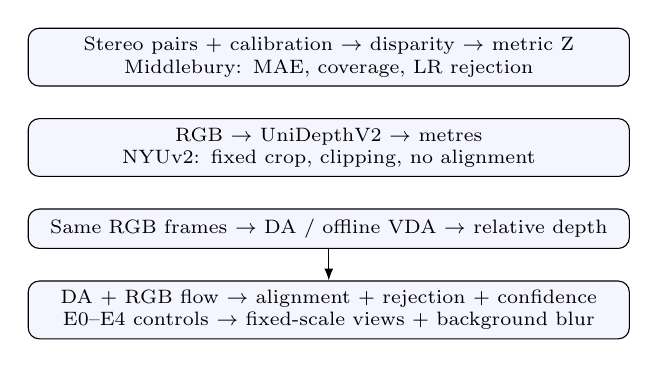
\begin{tikzpicture}[node distance=4mm, every node/.style={font=\scriptsize,align=center},
box/.style={draw,rounded corners,fill=blue!4,text width=7.4cm,minimum height=5mm},
arr/.style={-{Latex[length=1.5mm]}}]
\node[box] (s) {Stereo pairs + calibration $\rightarrow$ disparity $\rightarrow$ metric Z\\Middlebury: MAE, coverage, LR rejection};
\node[box,below=of s] (n) {RGB $\rightarrow$ UniDepthV2 $\rightarrow$ metres\\NYUv2: fixed crop, clipping, no alignment};
\node[box,below=of n] (v) {Same RGB frames $\rightarrow$ DA / offline VDA $\rightarrow$ relative depth};
\node[box,below=of v] (f) {DA + RGB flow $\rightarrow$ alignment + rejection + confidence\\E0--E4 controls $\rightarrow$ fixed-scale views + background blur};
\draw[arr] (v)--(f);
\end{tikzpicture}
\captionof{figure}{Three evaluation branches. Stereo and NYU have GT; the video branch has no depth GT. Only DA is modified by fusion.}
\end{minipage}\end{center}

\section{Methods and Evaluation}
\subsection{Stereo geometry and validity}
We run OpenCV 4.13 StereoSGBM on the 15 quarter-resolution Middlebury training pairs. Development uses Adirondack and Pipes; the other 13 scenes are separated from parameter selection. The all-15 summary is descriptive, not an official hidden-test score. Settings include a $3\times3$ block, uniqueness ratio 10, speckle window 100, speckle range 2, and prefilter cap 31. Search ranges follow the scene calibration.

The left disparity is $d=x_L-x_R$. OpenCV's signed fixed-point output is divided by 16. With quarter-resolution focal length $f$, baseline $B$ in millimetres, and calibration offset $c=\mathrm{doffs}$,
\begin{equation}
Z(d)=\frac{fB}{1000(d+c)}.
\label{eq:depth}
\end{equation}
Invalid matcher values, nonfinite outputs, and nonpositive Z are excluded from conditional errors. The optional extra left--right (LR) check samples the reverse match at the left correspondence and requires an in-bounds valid sample and residual at most 1 px. LR off/on retains the same original matching and OpenCV internal settings; it changes a mask, not retained disparities.

All-GT evaluation uses finite, positive GT disparities. We also report the supplied nonoccluded region. Coverage divides valid predictions by the fixed GT count. Disparity MAE and Z RMSE are conditional on valid predictions, whereas the supplementary bad-$1$ fraction counts invalid predictions as failures. Scene-level errors are macro averaged; coverage and bad-$1$ are pixel pooled.

\subsection{Pretrained metric and relative models}
UniDepthV2 ViT-S uses the official RGB-only \texttt{infer} path with predicted intrinsics and resolution level 0. Outputs are restored to $480\times640$. The official NYUv2 split~\cite{nyu} contains 795 training and 654 test images; three training-side examples were used for development checks. No model is locally trained. This inference-only use does not independently establish disjointness from upstream pretraining data.

NYU evaluation uses filled GT depths in metres, Python crop \texttt{[45:471,41:601]}, GT range $[0.001,10]$ m, and predictions clipped to that range. For each image's GT domain $\Omega$:
\begin{align}
\mathrm{AbsRel}&=\frac{1}{|\Omega|}\sum_{\Omega}\frac{|p-g|}{g},\\
\mathrm{RMSE}&=\sqrt{\frac{1}{|\Omega|}\sum_{\Omega}(p-g)^2},\\
\delta_1&=\frac{1}{|\Omega|}\sum_{\Omega}
\mathbf{1}\!\left[\max(p/g,g/p)<1.25\right].
\end{align}
Each metric is averaged equally over 654 images. No test scale or shift is fitted. These are course-protocol results, not claimed paper-score reproductions.

DA V2 Small processes frames independently; VDA Small uses official offline inference. Both use FP16, requested input size 364, and restored $640\times360$ outputs. The actual encoder spatial size is $364\times644$. The pinned repository clip contains 70 frames at 24 fps, not the requested 100. We process all 70 original frames without duplication and disclose this discrepancy; the user accepted this handling, which is not teacher approval. Tokyo, an optional repository example, supplies 100 frames at 15 fps for development. No self-recorded data are required.

\subsection{Causal flow-guided fusion}
Let $D_t$ be current DA and $H_{t-1}$ previous raw or fused depth. Backward flow warps history into current coordinates:
\begin{equation}
\widehat D_t=(1-w_t)D_t+w_t\,W(H_{t-1}).
\end{equation}
E0 returns DA. E1 blends at identical coordinates. E2 adds flow warping. E3 rejects out-of-bounds, photometrically inconsistent, and forward--backward (FB) inconsistent samples. E4 adds continuous confidence:
\begin{equation}
w_t=\alpha M_t\exp\!\left[-\frac{r_p}{.1}-\frac{r_f}{1}
-\frac{r_d}{.1}-\frac{r_e}{.1}\right].
\label{eq:confidence}
\end{equation}
Here $r_p$ is RGB residual, $r_f$ is FB residual in pixels, $r_d$ is absolute depth disagreement, and $r_e$ is a four-neighbor edge magnitude; the last two are divided by the current DA frame's P1--P99 span. This span only affects confidence, never raw predictions or per-frame display scaling. The hard gate requires $r_p\le.2$ and $r_f^2\le.01(\|F_b\|^2+\|W(F_f)\|^2)+.5$. These are heuristic weights, not calibrated probabilities.

Farneb\"ack uses pyramid scale .5, three levels, window 15, three iterations, polynomial neighborhood 5 and sigma 1.2. The frozen maximum weight is $\alpha=.70$. Recursive history uses $\widehat D_{t-1}$; pairwise uses $D_{t-1}$. First-frame outputs equal DA.

\subsection{Diagnostics and evidence boundaries}
Video colors use one fixed whole-clip P1--P99 range per model. E0--E4 share DA's range; VDA has its own. Relative zero values are valid finite outputs, not zero metres.

For common RGB/flow reference pixels, $T$ averages $\min(|D_t-W(D_{t-1})|/s,1)$ with fixed clip span $s$. Invalid pairs pay 1; valid-pair coverage is also reported. Departure measures mean $|\widehat D-D|/s$. Neither quantity is GT accuracy or a perceptual score. Real motion, flow error, and smoothing affect them. We inspected matched stills and consecutive contact sheets, with frame indices and ROI coordinates recorded; this is not full real-time playback. Test footage had been viewed before the renewed freeze, and supplementary analyses are post-hoc.

\widepage{jadeplant.png}{1}{Jadeplant diagnostic from unchanged StereoSGBM outputs. Gray denotes invalid or unavailable values. GT and prediction share display ranges; the last panel shows pre-rejection LR residual. The image-wide validity title differs from GT-domain coverage. Display clipping does not clip evaluation values.}
\section{Part 1: Stereo and Frame-Wise Baselines}
\subsection{LR reliability versus coverage}
Table~\ref{tab:stereo} shows that the optional custom LR check reduces conditional error but rejects many pixels. It cannot be described as correcting disparities. Across all-GT regions, 595,472 previously valid predictions are removed. Only 32.56\% of those exceed 1 px GT error; 67.44\% are within 1 px. Moreover, 82.20\% of rejections have no comparable right match. Lack of a reverse match is not proof that the left disparity was wrong.

\begin{center}\begin{minipage}{\linewidth}\centering
\captionof{table}{15-scene descriptive summary. Errors are scene macro averages on valid predictions; coverage and bad-$1$ are pooled over fixed GT pixels.}
\label{tab:stereo}
\small
\begin{tabular}{llrrrr}
\toprule
GT & LR & MAE px & Cov.\% & Z RMSE m & Bad-$1$\%\\
\midrule
All & off & 1.839 &75.63&.202&35.97\\
All & on &1.311&62.65&.150&44.73\\
Nonocc. &off&1.426&82.33&.169&28.05\\
Nonocc. &on&1.019&68.84&.122&37.82\\
\bottomrule
\end{tabular}
\end{minipage}\end{center}

On the 13 evaluation scenes, LR-on MAE is 1.337 px at 61.26\% coverage. The all-15 number includes development, so it should not replace this subset when discussing separation from tuning. All-GT contains 4,586,010 pixels, of which 2,873,146 remain after LR.

\subsection{Structure, tails, and metric conversion}
The eight-panel Jadeplant view reveals fragmented fine branches and clutter boundaries while preserving larger surfaces. Its conditional MAE is 3.524 px and GT-domain coverage 37.39\%; its P95 disparity error reaches 31.77 px. PianoL has 4.067 px MAE at 39.42\% coverage. A comparatively strong case, Teddy, has 0.414 px MAE and 72.96\% coverage. Figure~\ref{fig:boxes} shows why a mean alone is insufficient.

\panel{stereo_boxes.png}{1}{Selected scenes after LR: exact valid-pixel quantiles, quartile boxes, median lines and P5--P95 whiskers. Labels report GT-domain coverage. Disparity and depth have separate units; omitted tails remain in the evidence CSVs.\label{fig:boxes}}

Depth error follows an exact relation, with $K=fB/1000$:
\begin{equation}
Z(d)-Z(d^*)=\frac{-K(d-d^*)}{(d+c)(d^*+c)}.
\end{equation}
We verify this to floating-point precision; it is a correctness check, not a second method. Larger Z errors can arise despite moderate disparity errors. Pipes has 0.591 m Z RMSE and GT depths up to 8.566 m. All pixels beyond 6 m belong to development Pipes, so pooled distance trends confound scene and calibration with distance. Additional distance-bin distributions and coverage are provided with the reproducible analyses.

\widepage{nyu_cases.png}{1}{Two actual NYUv2 test cases, with matching GT/prediction scales within each row. Top: bookstore image 0088, the largest course AbsRel. Bottom: image 0033, where a modest depth RMSE coexists with missing thresholded monitor boundaries. Error is shown only inside the fixed course GT domain, capped at 2 m (top) and 0.5 m (bottom) for display; row-specific depth scales are labeled.}
\section{Part 2: Monocular Metric Depth}
\subsection{Course accuracy and protocol effects}
UniDepthV2 predicts finite positive depths over all 156,018,240 evaluated GT pixels. Table~\ref{tab:nyu} separates the required clipped protocol from an unclipped diagnostic on the same arrays. Upper clipping affects 554,689 pixels (0.3555\%) across 26 images; no lower clipping occurs. The 5.72\% RMSE decrease is a protocol effect, not a learned improvement.

\begin{center}\begin{minipage}{\linewidth}\centering
\captionof{table}{654-image equal-weight means; no alignment. The clipped row is the formal course result.}
\label{tab:nyu}
\begin{tabular}{lrrr}
\toprule
Preparation & AbsRel & RMSE m & $\delta_1$\\
\midrule
Unclipped diagnostic &.11224&.41666&.89311\\
Course-clipped &\textbf{.11078}&\textbf{.39282}&\textbf{.89478}\\
\bottomrule
\end{tabular}
\end{minipage}\end{center}

Pixel-pooled RMSE is 0.48305 m; it differs from the formal image-macro 0.39282 m because averaging square roots and taking a pooled square root are different operations. We retain the course definition.

\panel{nyu_distribution.png}{1}{Image-level distributions on all 654 test images. Quartile boxes and P5--P95 whiskers preserve the difference between typical cases and difficult tails; this is descriptive, not an independent-image significance analysis.}

Median image AbsRel is 0.09455, while its P95 is 0.23950. RMSE has median 0.30862 m, P95 0.94119 m, and maximum 2.01190 m. A single average therefore understates difficult scenes.

\subsection{Scale and boundary errors}
The median across per-image median prediction/GT ratios is 1.0370; the 5th--95th percentile interval is 0.8593--1.1965. These ratios diagnose bias and are never used to fit the test predictions. Mean signed error is only +0.0398 m, but positive and negative biases cancel. Image 0088 overestimates much of the bookstore, with median ratio 1.6812 and course AbsRel 0.6198. Living-room image 1208 has median ratio 0.6757 and underestimates much of the scene. Broad structure can be plausible even with substantial scale error.

Pooled RMSE by GT distance rises from 0.287 m at 1--2 m to 1.496 m at 6--10 m; the latter contains only 3.08\% of evaluated pixels. Nearer than 1 m, AbsRel is relatively high at 0.258. These groups mix objects and scenes and are not a distance-only experiment.

Our optional boundary diagnostic marks four-neighbor log-depth jumps above $\log(1.1)$, uses a 3-by-3 eroded GT domain, and allows 2 px matching tolerance. Pooled precision/recall/F1 are 0.758/0.400/0.523; macro F1 is 0.457. Prediction edges (1,290,091 pixels) are fewer than GT edges (2,295,868). These thresholds define a project diagnostic, not a published benchmark replication.

Image 0033 has RMSE 0.1475 m but boundary F1 zero: the broad room/monitor structure is present while the selected depth discontinuities are too smooth. Conversely, a largely planar whiteboard image 0042 has only 75 GT edge pixels and low RMSE 0.0548 m; zero F1 there does not imply the whole depth map fails. Mirror-region discrepancies in 1293 and 1354 require caution because filled sensor GT does not independently certify the physical depth of reflections. Thirteen diagnostic images were inspected, including distribution extremes and boundary cases.

\widepage{video.png}{1}{Identical rollercoaster ROI at frames 14--16. DA changes bright--dark--bright over the train and nearby track. E4 leaves much of that change; VDA is more stable in this window. Passenger/seat gaps remain merged. All outputs are relative; VDA's colors use a different fixed whole-clip range, not shared metres.}
\section{Video Baselines and Fusion Results}
\subsection{Frame-wise DA versus offline VDA}
DA recovers recognizable tracks, coarse supports, and separation from the sky. The inspected large supports do not all vanish or flicker; the more precise failure is incomplete fine structure and a localized train/track color fluctuation. VDA reduces the latter at frames 14--19 but still merges small passenger and seat details. Late frames 64--69 retain jagged or filled gaps. No measured response-latency claim is made.

The official offline implementation uses 32-frame inputs, a 22-frame step, keyframe reuse and eight-frame overlap interpolation. The 70-frame clip is processed in four windows with final-frame padding, then truncated back to 70 outputs. The first ten input positions reuse selected earlier keyframes; this is not simply four disjoint batches. Two inspected interpolation regions, frames 24--31 and 46--53, show no prominent color seam. These observations do not establish consistency over arbitrarily long video.

\begin{center}\begin{minipage}{\linewidth}\centering
\captionof{table}{Recorded model inference, excluding loading, I/O, evaluation and rendering. GPU peak is PyTorch allocated memory; reserved memory is given in text.}
\label{tab:resources}
\small
\begin{tabular}{lrrr}
\toprule
Model & ms/output & FPS & Peak MiB\\
\midrule
DA V2 Small &36.697&27.250&268.98\\
VDA Small offline &74.235&13.471&2386.35\\
UniDepthV2 ViT-S &47.897&20.878&401.95\\
\bottomrule
\end{tabular}
\end{minipage}\end{center}

Hardware is an RTX 4060 Laptop GPU (8 GB), Windows 11, PyTorch 2.10.0+cu128, CUDA 12.8 and FP16. Reserved peaks are 304, 3164 and 456 MiB respectively. UniDepth uses encoder size $434\times574$, batch one; DA uses $364\times644$, batch one; VDA uses 32-frame windows at that spatial size. VDA ms/output divides clip-total inference time by output frames; FPS is its reciprocal, not causal latency. Stereo is CPU-only: the current Adirondack run takes 0.104 s for one measured pair after one warmup at $718\times496$, which is not a benchmark.

\subsection{E0--E4 main comparison}
\begin{center}\begin{minipage}{\linewidth}\centering
\captionof{table}{Same DA scale and public reference pixels within each clip. $D$ is departure from current DA, not GT error. All reference-pair coverages equal 1.}
\label{tab:main}
\small
\begin{tabular}{lrrrr}
\toprule
&\multicolumn{2}{c}{Tokyo}&\multicolumn{2}{c}{Rollercoaster}\\
Method &$T$&$D$&$T$&$D$\\
\midrule
E0&.005168&0&.014708&0\\
E1&.002950&.005868&.015586&.092337\\
E2&.002647&.006097&.004983&.011845\\
E3&.002609&.005916&.004653&.009546\\
E4&.003439&.002817&.012364&.001561\\
\bottomrule
\end{tabular}
\end{minipage}\end{center}

On rollercoaster, E1 worsens $T$ and creates broad support ghosts. E2 alignment markedly reduces those ghosts; E3 further limits inappropriate history but can yield mottled train interiors. E4 retains clearer current-frame contours yet smooths less. Its $T$ is 15.93\% below DA, but it is not the lowest-$T$ variant. Tokyo shows the same contour-versus-smoothing tradeoff, while E1's lower $T$ there illustrates that a small diagnostic value can coexist with bad outlines.

Reference pixels cover 89.20\% of rollercoaster and 98.17\% of Tokyo adjacent-pair pixels, excluding some difficult flow/occlusion regions. E4's estimated rollercoaster pipeline speed is 6.534 FPS from separate recorded DA (2.569 s), flow (6.628 s), and fusion (1.517 s) stages. This is a sum, not a repeated end-to-end measurement. VDA has $T=.011590$ under its own span; raw units differ, so it is not a common-unit accuracy ranking.

\widepage{modules.png}{1}{Module comparison at rollercoaster frames 15 and 35. E1 accumulates repeated supports. Flow alignment in E2 limits this spread; E3 rejects more history but produces localized mottling. E4 resembles the current DA silhouette more closely. All four share DA's fixed scale.}
\section{Controlled Supplementary Experiments}
\subsection{History source: pairwise versus recursive}
For each E1--E4 variant, only the history source changes. Pairwise uses the preceding raw prediction and still uses history; E0 is the actual no-history control. Inputs, optical flow, thresholds and weight formula remain fixed. E4's numeric weights can change because its depth-confidence term depends on history.

\begin{center}\begin{minipage}{\linewidth}\centering
\captionof{table}{Recursive reduction in $T$ relative to pairwise. Lower $T$ alone does not establish better shape or motion response.}
\small
\begin{tabular}{lrrrr}
\toprule
Clip &E1&E2&E3&E4\\
\midrule
Tokyo &30.77\%&35.84\%&36.09\%&15.28\%\\
Rollercoaster &7.84\%&44.22\%&45.23\%&0.95\%\\
\bottomrule
\end{tabular}
\end{minipage}\end{center}

Recursive E1 makes wider repeated contours than pairwise (Fig.~\ref{fig:history}). E2 recursive leaves softer passenger contours in the inspected rollercoaster window; both E3 histories remain locally mottled. E4's pairwise/recursive images are nearly indistinguishable there. Its rollercoaster $T$ changes only from .0124824 to .0123643. Departure slightly decreases (.001638 to .001561), which is possible because history also changes depth confidence. Accumulation is therefore neither uniformly useful nor uniformly more distant from DA.

\panel{history.png}{1}{Frame 15: recursive E1 has broad multiframe ghosts; pairwise confines the blend to two frames but does not fully solve misalignment. Both are worse than current DA in rollercoaster $T$.\label{fig:history}}

\subsection{Four soft-confidence removals}
We remove one term at a time from Eq.~\ref{eq:confidence}, retaining all hard gates and the same recursive history rule. This identifies marginal effects conditional on the other components; it is not a full interaction study.

\begin{center}\begin{minipage}{\linewidth}\centering
\captionof{table}{Leave-one-out E4 on each clip. $T$ decreases for every removal, while departure from DA increases.}
\small
\begin{tabular}{lrrrr}
\toprule
&\multicolumn{2}{c}{Tokyo}&\multicolumn{2}{c}{Rollercoaster}\\
Setting &$T$&$D$&$T$&$D$\\
\midrule
Full&.003439&.002817&.012364&.001561\\
No photo&.003200&.003433&.011977&.001843\\
No flow&.003354&.003013&.012113&.001749\\
No depth&.003243&.003523&.010948&.002569\\
No edge&.003330&.003067&.011028&.002719\\
\bottomrule
\end{tabular}
\end{minipage}\end{center}

Photo has the largest $T$ effect on Tokyo; depth and edge have larger effects on rollercoaster. Full E4 and each removal look very similar in the inspected contact sheets. We do not claim that each term visibly improves quality. Their measured role is to constrain temporal smoothing, and results depend on the clip.

\subsection{Development fusion strength}
With all other settings fixed, Tokyo $\alpha=.50/.70/.85$ yields $T=.003899/.003439/.003101$ and departure $.001844/.002817/.003741$. Increasing history reduces $T$ while changing current DA more. Matched pedestrian windows 28--33 and 60--65 reveal only subtle differences, with no clear additional harm from .85. The retained .70 setting is a conservative existing choice, not a demonstrated optimum. Test results were not used to retune it. Correlated frames do not supply independent trials, and none of these post-hoc controls is presented as a new blind test.

\widepage{application.png}{1}{Depth-aware blur at frames 0 and 35. Old transition thresholds blur some train/track/support detail. The lower thresholds preserve more of it; DA and E4 with the same new setting appear nearly identical. Crops use the same RGB coordinates, and no semantic foreground labels are used.}
\section{Application, Failure Cases, and Conclusions}
\subsection{Separate application and depth effects}
Our application seeks to keep passengers, cars, tracks and supports clear while blurring distant background. Normalize relative inverse-depth-like values once using DA's full-clip range $[0,2.34975]$, producing $q$. With $u=\mathrm{clip}((q-a)/(b-a),0,1)$, the blur weight is
\begin{equation}
w_{\rm blur}=1-(3u^2-2u^3).
\end{equation}
The rendered image blends RGB and a Gaussian-blurred copy with $\sigma=5$ px. The old transition is $(a,b)=(.45,.70)$; the new transition is $(.10,.30)$. Lower thresholds keep more intermediate predicted depths sharp. This is depth thresholding, not object recognition, and cannot guarantee semantic foreground protection.

\begin{center}\begin{minipage}{\linewidth}\centering
\captionof{table}{All 70 frames. The same depth is compared across thresholds and the same threshold across DA/E4. Fractions describe effect strength, not foreground accuracy.}
\small
\begin{tabular}{lrr}
\toprule
Setting &Mean blur weight &Fully sharp \%\\
\midrule
DA, old &.850078&8.4360\\
E4, old &.850221&8.4117\\
DA, new &.754081&23.7014\\
E4, new &.754077&23.7020\\
\bottomrule
\end{tabular}
\end{minipage}\end{center}

Changing thresholds with DA fixed produces mean absolute RGB change 4.2543 on the 0--255 scale. Changing DA to E4 under the new thresholds changes only 0.002984. The visible benefit is primarily from thresholds; it is not evidence that E4 improves the application. Clouds and late background trees remain blurred in inspected images, but thin boundaries retain softening or halos. The new thresholds were chosen after viewing the test clip and are explicitly a post-hoc demonstration setting.

\subsection{Difficult cases actually present}
\paragraph{Thin clutter and occlusion.}
Middlebury Jadeplant contains thin branches, leaves and a repeated crate pattern. Predictions are fragmented and LR removes substantial coverage. The conditional error improvement must be reported alongside missing pixels. Better correspondence or boundary-aware matching could help, but this study does not prove such a remedy.

\paragraph{Metric scale despite plausible structure.}
NYU bookstore 0088 retains shelf structure but substantially overpredicts depth; the clipped RMSE is 2.0119 m. A single-image prior does not guarantee scene-specific scale. A future global calibration would have to be fitted on training/development data and frozen before testing.

\paragraph{Smooth boundaries despite low global error.}
NYU monitor case 0033 has modest RMSE but no matches under our chosen edge criterion. This motivates boundary-aware evaluation separately from average depth error. A refinement should avoid copying RGB texture into geometry.

\paragraph{Motion, ghosts and unresolved detail.}
Rollercoaster frames 14--19 expose color changes and small passenger/seat gaps. Unwarped history creates support ghosts; aligned history can soften edges; confidence weighting leaves some fluctuations. VDA is more color-stable in this window but does not restore all fine structures. A stronger flow model or an improved occlusion model is a future experiment, not an established fix.

\subsection{Conclusions and reproducibility}
Calibrated conversion is correct, but correspondence errors and coverage dominate stereo quality. UniDepthV2 obtains useful metric predictions under the required protocol, with uneven scale and boundary performance. VDA improves an observed temporal fluctuation at higher inference memory cost. Flow fusion offers a controllable tradeoff: strong smoothing lowers $T$ but can retain stale structure; E4 is more conservative, with residual changes and CPU flow cost. The application study establishes a threshold effect, not a clear benefit from E4.

The repository includes manifests, model revisions, raw-output export, verifiers, analysis scripts and compact report evidence. Each analysis records its inspected samples, settings, source hashes, statistics and limitations. Full arrays and large media remain local. No training, metric-video or streaming claim is made; the supplied short clip cannot support long-video generalization. The 70/100-frame discrepancy remains disclosed.

This sample report is intended for author review. Course ownership remains A (Qinchuan XIAO): geometry/data/evaluation, and B (Jun Yu Eugene YIP): models/video. Implementation, execution and analysis were assisted by Codex; this does not certify either member's independent acceptance. Canvas submission and publication are separate actions.

\clearpage
{\small\bibliographystyle{ieeenat_fullname}\bibliography{references}}
\end{document}
